\documentclass[t,dvipsnames]{beamer}

\setbeamertemplate{navigation symbols}{}
\useinnertheme{circles}
% \usecolortheme{crane}

% \usepackage[T1]{fontenc}
\usepackage[utf8]{inputenc}
% \usepackage[polish]{babel}
\usepackage[british]{babel}

\usepackage[adobe-utopia]{mathdesign}
\usepackage[series=z]{libgreek}
\usepackage{tgpagella}
\usepackage[textwidth=4cm]{todonotes}
\usepackage{minted}
\usemintedstyle{colorful}
% \usemintedstyle{autumn}
% \usemintedstyle{vs}
\usepackage{tikz}
\usetikzlibrary{matrix,arrows,calc}
\tikzset{every scope/.style={>=angle 60,thick}}

\author{Marcin Szamotulski}
\institute{\insertlogo{
\includegraphics[height=1cm]{iohk-logo.png}}}
\title{Typed Protocol Pipelining}

\setbeamertemplate{frametitle}[default][center]

\begin{document}
\begin{frame}
    \titlepage
\end{frame}

\begin{frame}
  \frametitle{Ping Pong Protocol}
  \vspace{1cm}
  \begin{figure}
    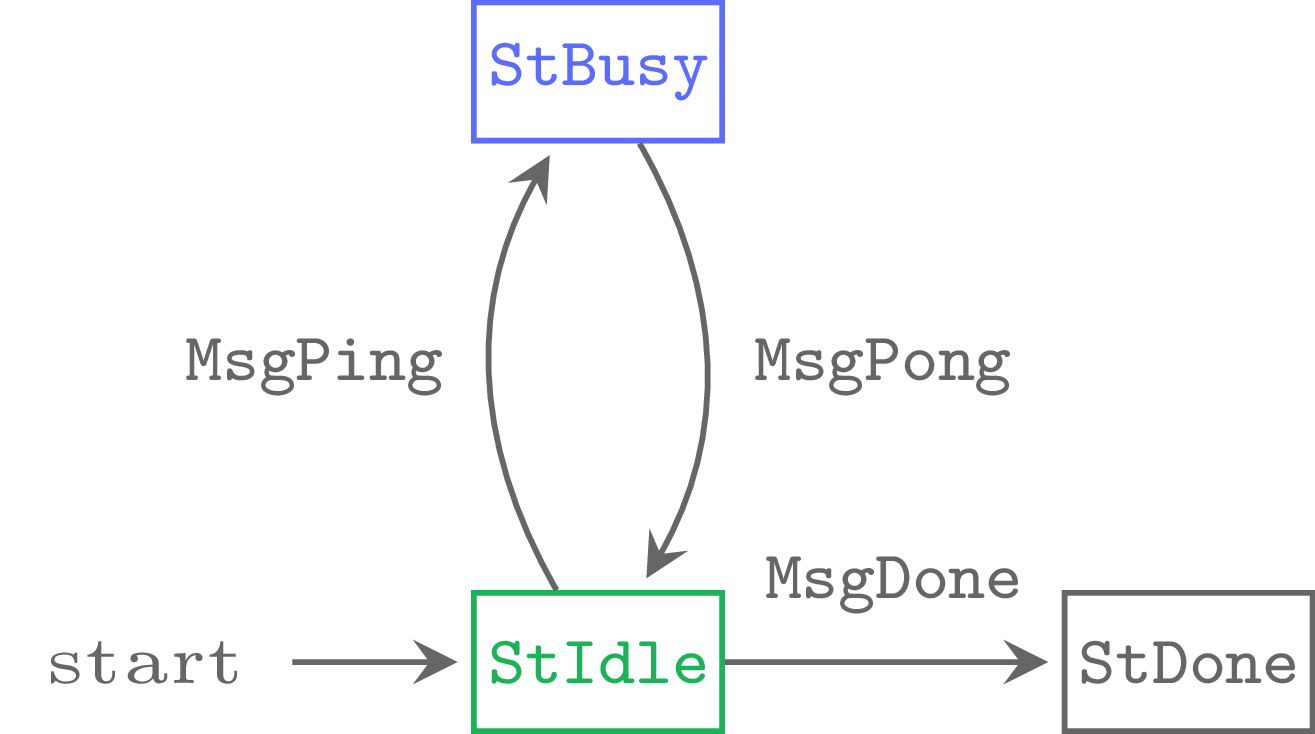
\includegraphics{../images/ping-pong-0.png}
    \caption{PingPong protocol state diagram}
  \end{figure}
\end{frame}

\begin{frame}
  \frametitle{Protocol pipelining}

  \vspace{1cm}
  \begin{figure}
    \begin{minipage}{.4\textwidth}
      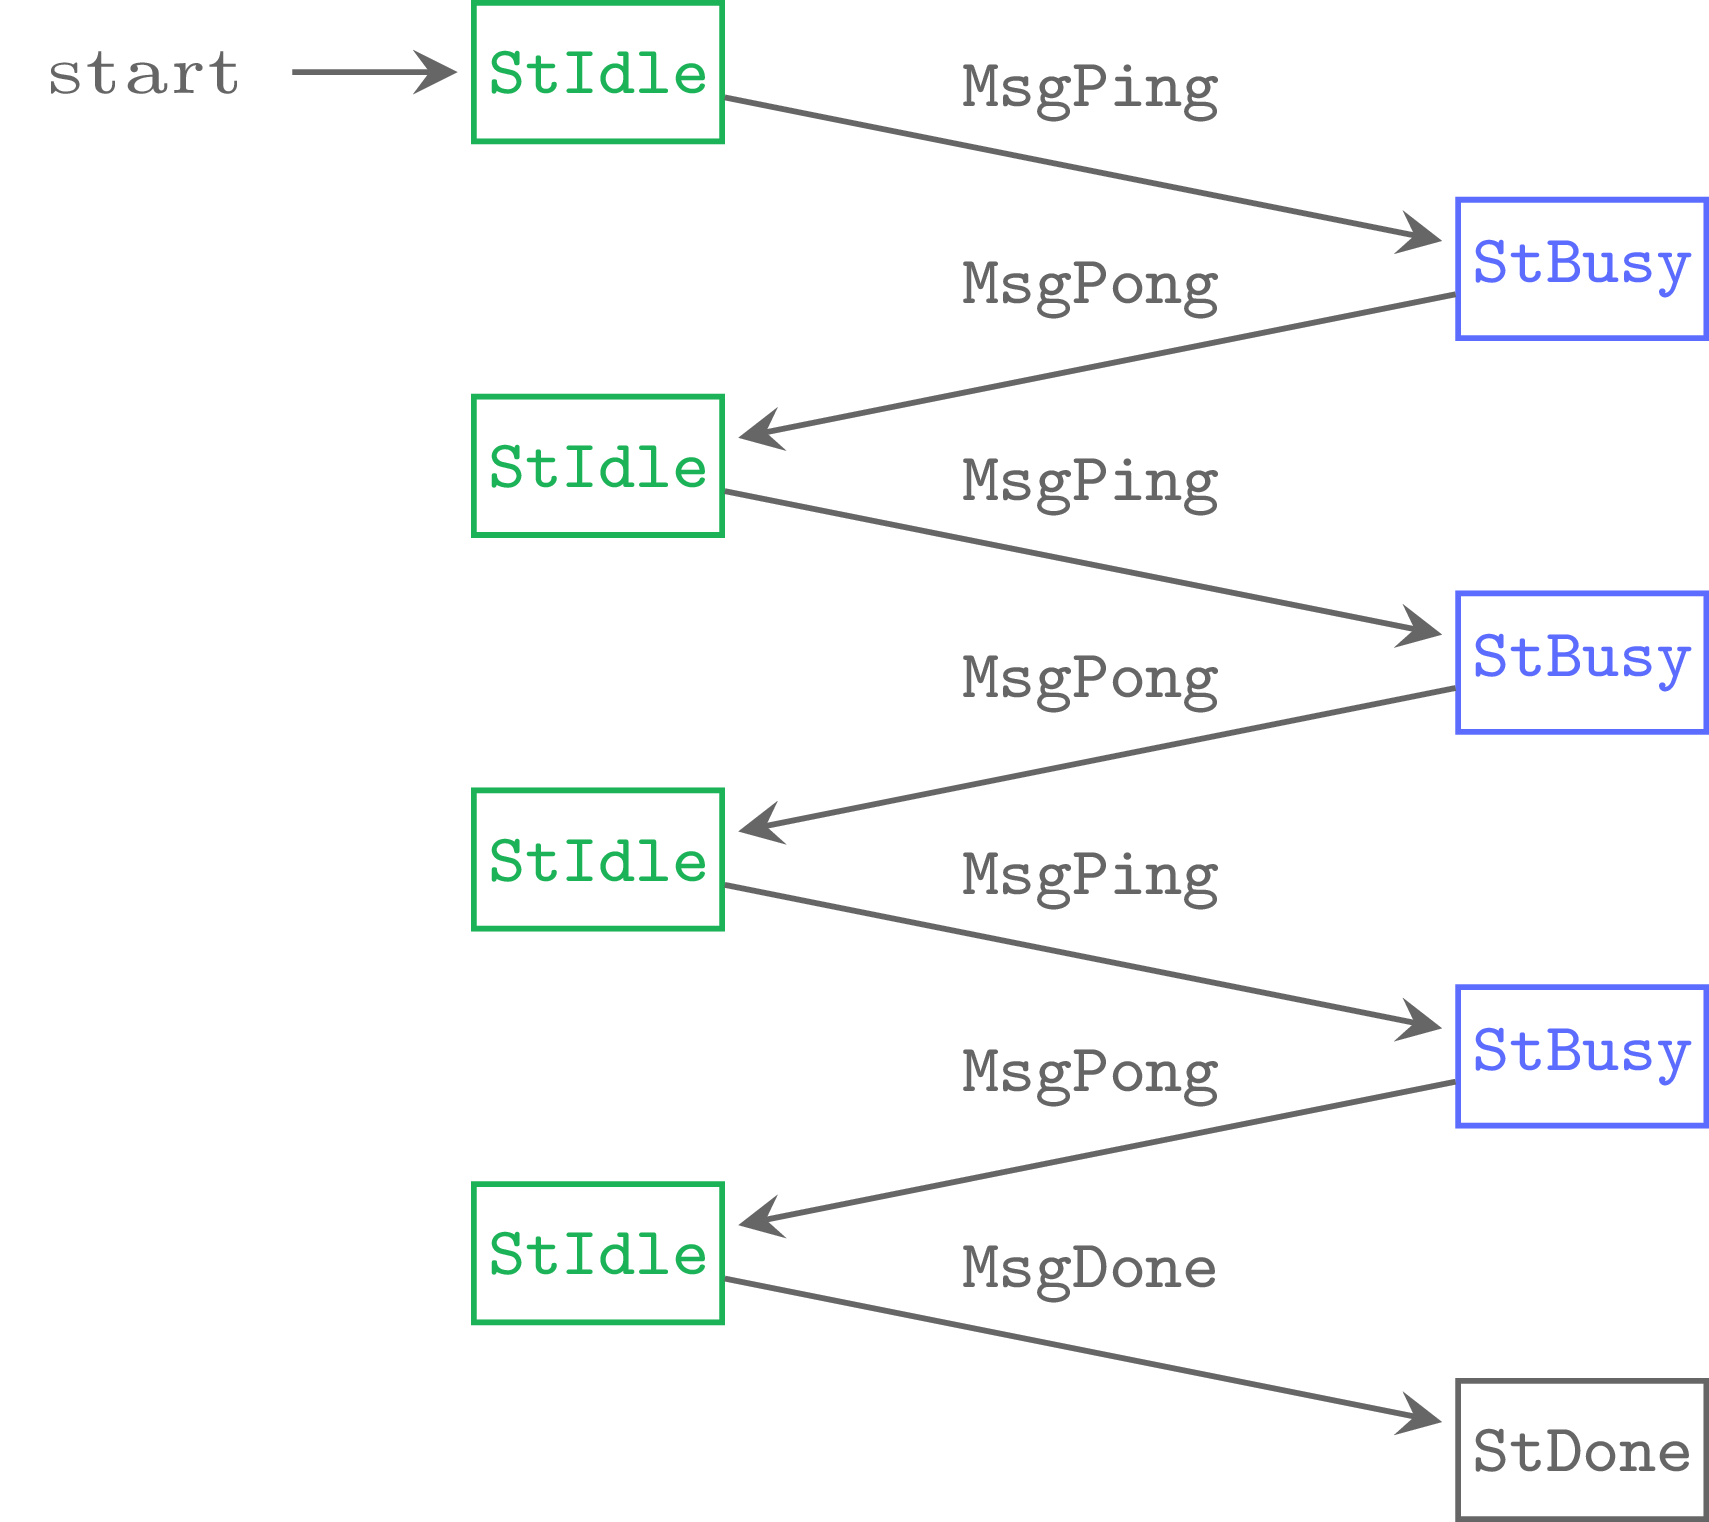
\includegraphics{../images/ping-pong-1.png}
      \vspace{2cm}
    \end{minipage}
    \begin{minipage}{.4\textwidth}
      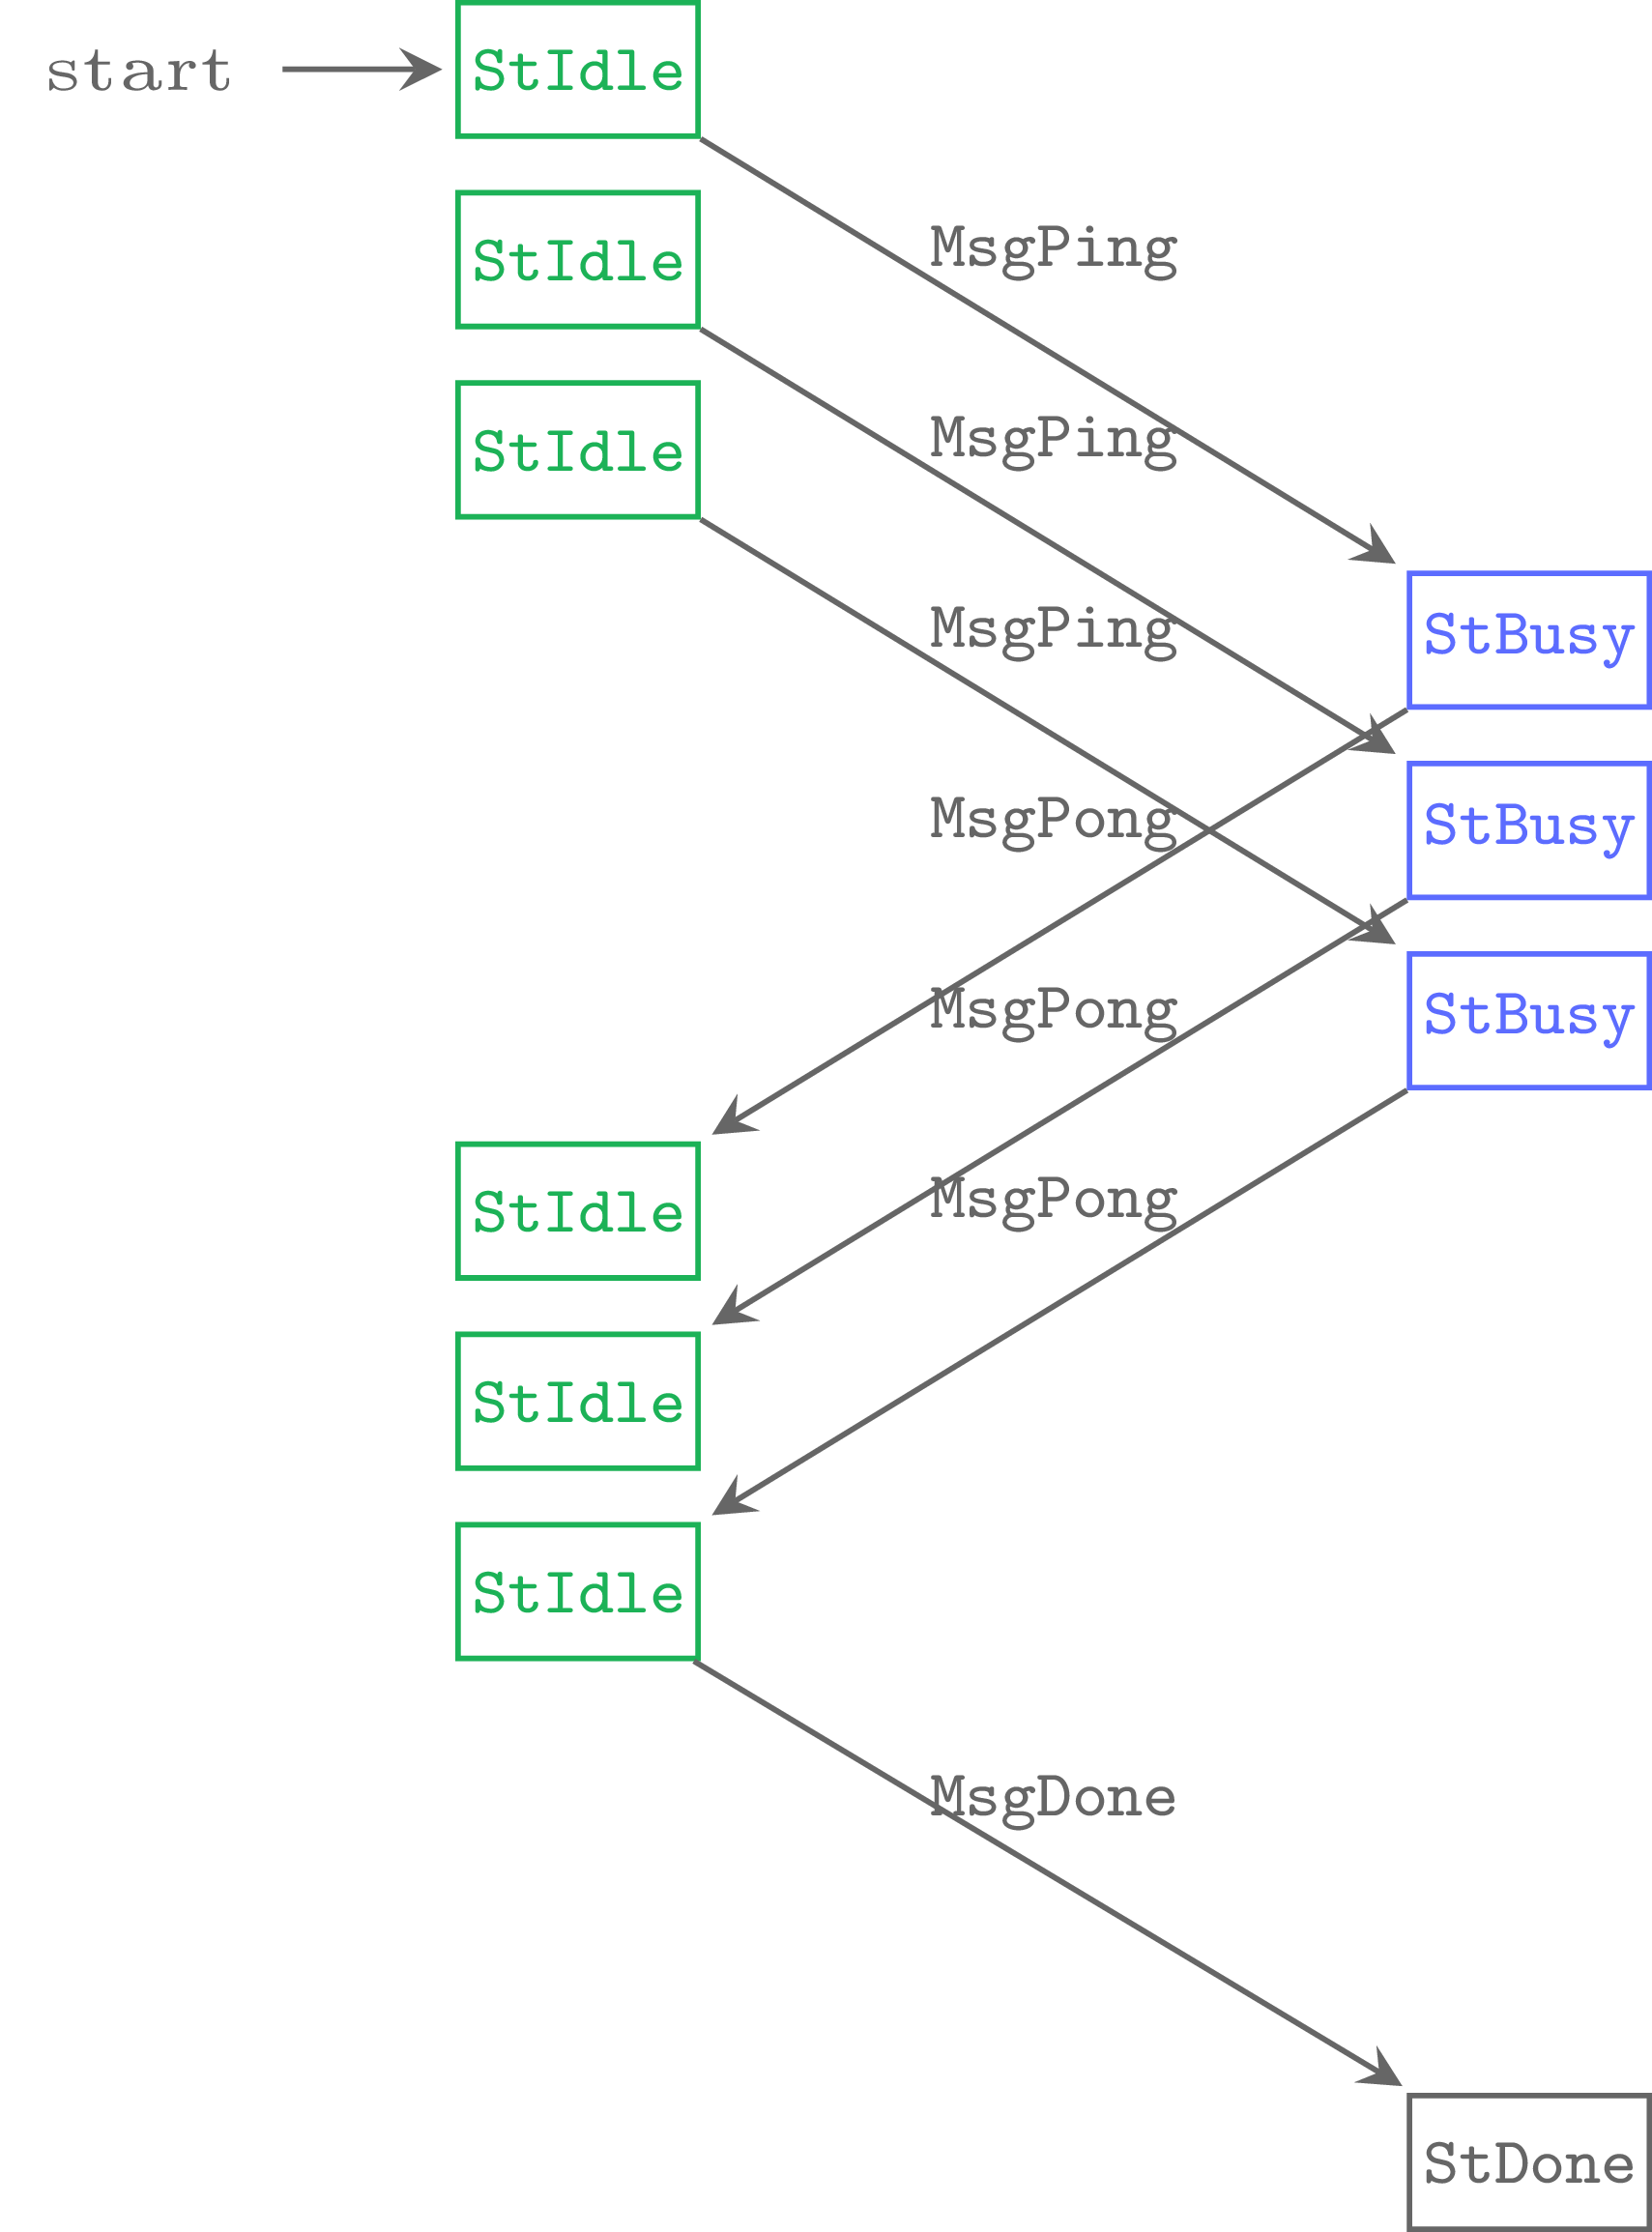
\includegraphics{../images/ping-pong-2.png}
    \end{minipage}
    \caption{non-pipelined vs pipelined ping pong client}
  \end{figure}

\end{frame}

\begin{frame}
  \frametitle{Protocol pipelining}
  \vspace{1cm}
  \begin{itemize}
    \item \textbf{latency hidding}
    \item \textbf{network utilisation}
        \textit{network is utilised best when constant pressure is
         applied to avoid shrinking of the tcp window (e.g. tcp flow control
         mechanism).  Network utilisation is a balance between keeping the most
         constrained resource busy - but only just - too busy and delay increases and
         application responsiveness can drop.}
  \end{itemize}

  \begin{itemize}
    \item pipelined transitions are no longer a continous flow of matching transitions (i.e. composition of state transitions).
    \item pipelining must keep relative order of reqests and response
      transitions, but can mix both groups.
  \end{itemize}
\end{frame}

\begin{frame}[fragile]
  \frametitle{Towards non-pipelined protocol description}
  \begin{columns}[t]
    \begin{column}{1.0\textwidth}
      \begin{minted}[stripall,bgcolor=NavyBlue!5!white,fontsize=\tiny]{haskell}
data PingPong where
  StIdle :: PingPong
  StBusy :: PingPong
  StDone :: PingPong

data MessageSimplePingPong (st :: PingPong)
                           (st' :: PingPong) where
  MsgSimplePing :: MessageSimplePingPong StIdle StBusy
  MsgSimplePong :: MessageSimplePingPong StBusy StIdle
  MsgSimpleDone :: MessageSimplePingPong StIdle StDone

data SimplePingPongClient (st :: PingPong) a where
  SendMsg    :: MessageSimplePingPong StIdle st
             -> (SimplePingPongClient st a)
             -> SimplePingPongClient StIdle a

  RecvMsg    :: (MessageSimplePingPong StBusy StIdle
                  -> (SimplePingPongClient StIdle a))
             -> SimplePingPongClient StBusy a

  ClientDone :: a
             -> SimplePingPongClient StDone a
      \end{minted}
    \end{column}
  \end{columns}
\end{frame}

\begin{frame}[fragile]
  \frametitle{Towards non-pipelined protocol description}
  \begin{columns}[t]
    \begin{column}{1.0\textwidth}
      \begin{minted}[stripall,bgcolor=NavyBlue!5!white,fontsize=\tiny]{haskell}
simplePingPongClient :: a -> SimplePingPongClient StIdle a
simplePingPongClient a =
   SendMsg MsgSimplePing
 $ RecvMsg $ \MsgSimplePong ->
   SendMsg MsgSimplePing
 $ RecvMsg $ \MsgSimplePong ->
   SendMsg MsgSimplePing
 $ RecvMsg $ \MsgSimplePong ->
   SendMsg MsgSimpleDone
 $ ClientDone a
      \end{minted}
    \end{column}
  \end{columns}
\end{frame}

\begin{frame}[fragile]
  \frametitle{Towards pipelined protocol description}
      \begin{minted}[stripall,bgcolor=NavyBlue!5!white,fontsize=\tiny]{haskell}
data N = Z | S N

data SimplePipelinedPingPongClient (st :: PingPong)
                                   (n :: N) c a where
  PipelinedSendMsg
    :: MessageSimplePingPong StIdle st
    -> PingPongReceiver              StBusy StIdle c
    -> SimplePipelinedPingPongClient StIdle (S n) c a
    -> SimplePipelinedPingPongClient StIdle    n  c a

  CollectResponse
    :: (c -> SimplePipelinedPingPongClient StIdle n c a)
    -> SimplePipelinedPingPongClient StIdle (S n) c a

  SendMsgDone
    :: MessageSimplePingPong StIdle StDone
    -> SimplePipelinedPingPongClient StDone Z c a
    -> SimplePipelinedPingPongClient StIdle Z c a

  PipelinedDone
    :: a
    -> SimplePipelinedPingPongClient StDone Z c a

data PingPongReceiver (st :: PingPong)
                      (st' :: PingPong) c where
  RecvPipelinedMsg
    :: (MessageSimplePingPong StBusy StIdle -> c)
    -> PingPongReceiver StBusy StIdle c
      \end{minted}
\end{frame}

\begin{frame}[fragile]
  \frametitle{Towards pipelined protocol description}

  \begin{minted}[stripall,bgcolor=NavyBlue!5!white,fontsize=\footnotesize]{haskell}
simplePipelinedPingPongClient
   :: a -- ^ fixed result, for simplicity
   -> c -- ^ fixed collected value, for simplicity
   -> SimplePipelinedPingPongClient StIdle Z c a
simplePipelinedPingPongClient a c =
   PipelinedSendMsg
     MsgSimplePing
     (RecvPipelinedMsg $ \MsgSimplePong -> c)
     (PipelinedSendMsg
       MsgSimplePing
       (RecvPipelinedMsg $ \MsgSimplePong -> c)
       (CollectResponse $ \_c0 ->
         CollectResponse $ \_c1 ->
           SendMsgDone MsgSimpleDone $
             PipelinedDone a
       )
     )
  \end{minted}
\end{frame}

\begin{frame}[fragile]
  \frametitle{Towards pipelined protocol description}
  \vspace{2cm}
  Branching in \texttt{PipelinedSendMsg} requires that the interpretation of
  \texttt{SimplePipelinedPingPongClient} needs to concurrent execution: 
    \begin{minted}[stripall,bgcolor=NavyBlue!5!white,fontsize=\footnotesize]{haskell}
PipelinedSendMsg
  :: MessageSimplePingPong StIdle st
  -> PingPongReceiver              StBusy StIdle c
  -> SimplePipelinedPingPongClient StIdle (S n) c a
  -> SimplePipelinedPingPongClient StIdle    n  c a
    \end{minted}
\end{frame}

\begin{frame}[fragile]
  \frametitle{Typed Protocol Description}
  \begin{minted}[stripall,bgcolor=NavyBlue!5!white,fontsize=\footnotesize]{haskell}
data PeerRole = AsClient | AsServer

type PeerHasAgency :: PeerRole -> ps -> Type
data PeerHasAgency    pr          st where
    ClientAgency :: !(ClientHasAgency st)
                 -> PeerHasAgency AsClient st
    ServerAgency :: !(ServerHasAgency st)
                 -> PeerHasAgency AsServer st

type WeHaveAgency   (pr :: PeerRole) st =
    PeerHasAgency pr  st

type TheyHaveAgency (pr :: PeerRole) st =
    PeerHasAgency (FlipAgency pr) st

type family FlipAgency (pr :: PeerRole) where
    FlipAgency AsClient = AsServer
    FlipAgency AsServer = AsClient
  \end{minted}
\end{frame}

\begin{frame}[fragile]
  \frametitle{Typed Protocol Description}
  \begin{minted}[stripall,bgcolor=NavyBlue!5!white,fontsize=\footnotesize]{haskell}
class Protocol ps where
  data Message ps (st :: ps) (st' :: ps)
  data ClientHasAgency (st :: ps)
  data ServerHasAgency (st :: ps)
  data NobodyHasAgency (st :: ps)

  exclusionLemma_ClientAndServerHaveAgency
    :: forall (st :: ps).  ClientHasAgency st
                        -> ServerHasAgency st
                        -> Void

  exclusionLemma_NobodyAndClientHaveAgency
    :: forall (st :: ps).  NobodyHasAgency st
                        -> ClientHasAgency st
                        -> Void

  exclusionLemma_NobodyAndServerHaveAgency
    :: forall (st :: ps).  NobodyHasAgency st
                        -> ServerHasAgency st
                        -> Void
  \end{minted}
\end{frame}

\begin{frame}
  \frametitle{Exclude Lemmas}
  \begin{figure}
    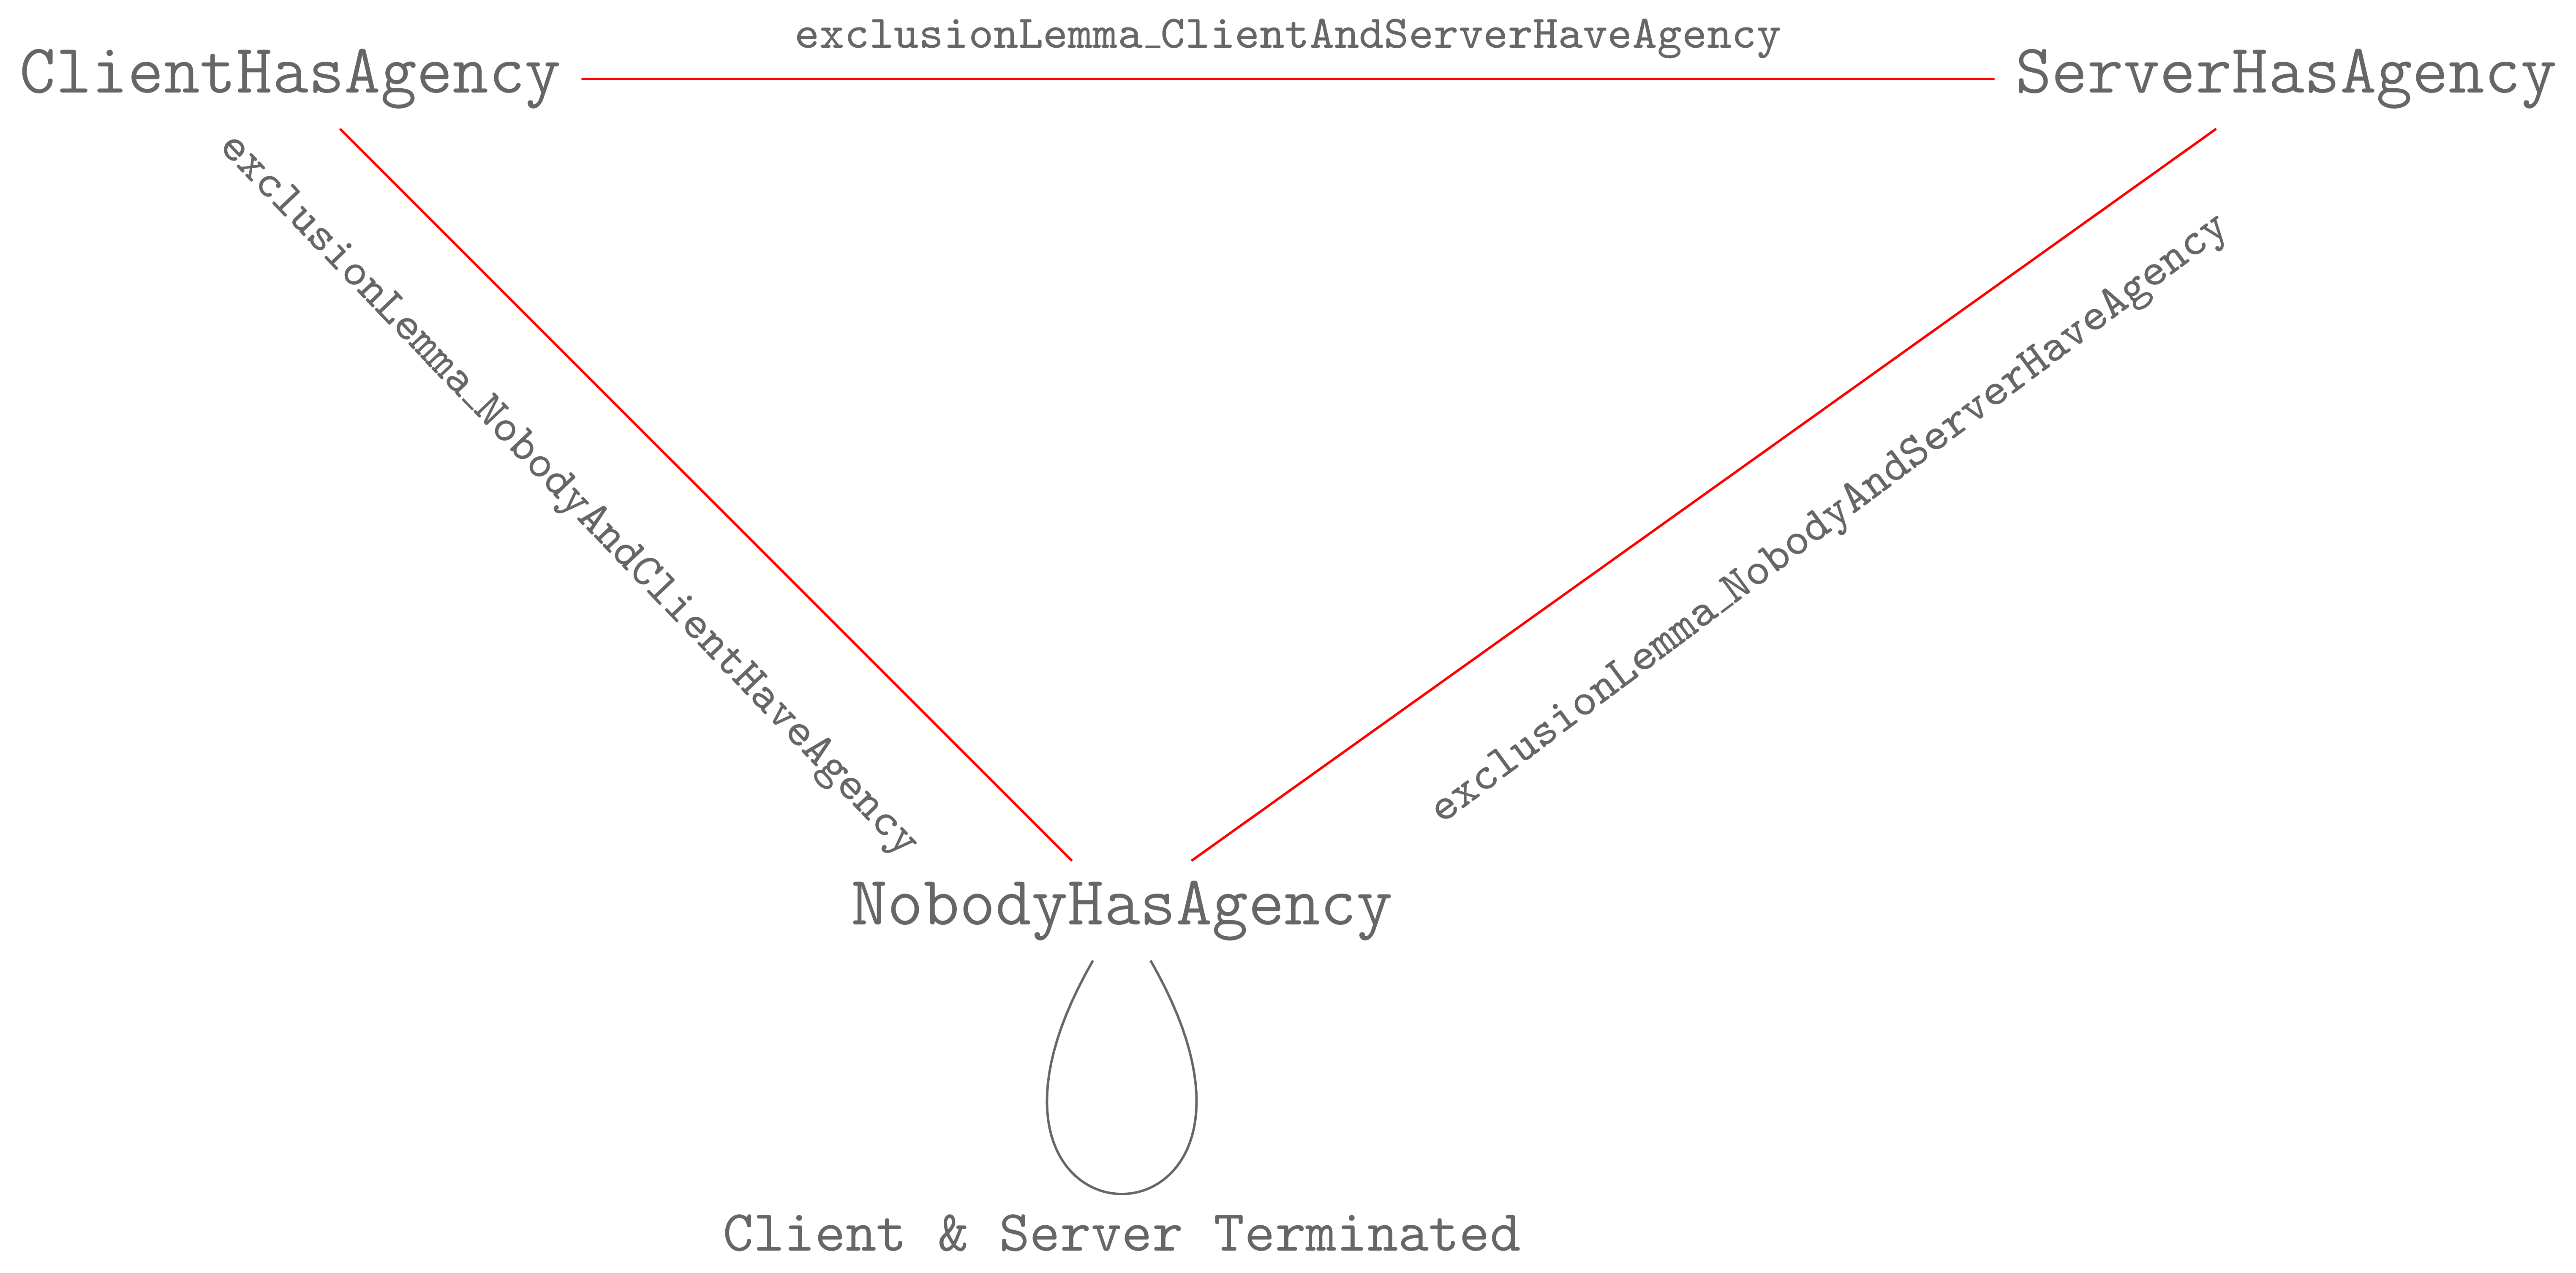
\includegraphics[width=11cm]{../images/exclusion_lemmas.png}
  \end{figure}
\end{frame}

\begin{frame}[fragile]
  \frametitle{Ping Pong Protocol}

  \begin{minted}[stripall,bgcolor=NavyBlue!5!white,fontsize=\footnotesize]{haskell}
instance Protocol PingPong where
  data Message PingPong from to where
    MsgPing :: Message PingPong StIdle StBusy
    MsgPong :: Message PingPong StBusy StIdle
    MsgDone :: Message PingPong StIdle StDone

  data ClientHasAgency st where
    TokIdle :: ClientHasAgency StIdle
  data ServerHasAgency st where
    TokBusy :: ServerHasAgency StBusy
  data NobodyHasAgency st where
    TokDone :: NobodyHasAgency StDone

  exclusionLemma_ClientAndServerHaveAgency TokIdle tok =
    case tok of {}
  exclusionLemma_NobodyAndClientHaveAgency TokDone tok =
    case tok of {}
  exclusionLemma_NobodyAndServerHaveAgency TokDone tok =
    case tok of {}
  \end{minted}
\end{frame}

\begin{frame}[fragile]
  \frametitle{Typed Protocol Pipelining}
  \begin{minted}[stripall,bgcolor=NavyBlue!5!white,fontsize=\footnotesize]{haskell}
data Trans ps where
    Tr :: forall ps. ps -> ps -> Trans ps

data Queue ps where
  Empty :: Queue ps
  Cons  :: Trans ps -> Queue ps -> Queue ps

type  (<|) :: Trans ps -> Queue ps -> Queue ps
type a <| as = Cons a as
infixr 5 <|

type (|>) :: Queue ps -> Trans ps -> Queue ps
type family as |> b where
     Empty     |> b = Cons b Empty
     (a <| as) |> b = a <| (as |> b)
infixr 5 |>
  \end{minted}
\end{frame}

\begin{frame}[fragile]
  \frametitle{Typed Protocol Pipelining}
  \framesubtitle{non-pipelined primitives}
  \begin{minted}[stripall,bgcolor=NavyBlue!5!white,fontsize=\footnotesize]{haskell}
data Pipelined = NonPipelined | Pipelined
data Peer ps pr pl st q m a where
  Effect
    :: m (Peer ps pr pl q st m a)
    ->    Peer ps pr pl q st m a
  Yield
    :: !(WeHaveAgency pr st)
    -> Message ps st st'
    -> Peer ps pr pl Empty st' m a
    -> Peer ps pr pl Empty st  m a
  Await
    :: !(TheyHaveAgency pr st)
    -> (forall st'. Message ps st st'
        -> Peer ps pr pl Empty st' m a)
    -> Peer     ps pr pl Empty st  m a
  Done
    :: !(NobodyHasAgency st)
    -> a
    -> Peer ps pr pl Empty st m a
  \end{minted}
\end{frame}

\begin{frame}[fragile]
  \frametitle{Typed Protocol Pipelining}
  \framesubtitle{pipelined primitives}
  \begin{minted}[stripall,bgcolor=NavyBlue!5!white,fontsize=\footnotesize]{haskell}
-- | Pipelined a message
YieldPipelined
  :: !(WeHaveAgency pr st)
  -> Message ps st st'
  -> Peer ps pr 'Pipelined (q |> Tr st' st'') st'' m a
  -> Peer ps pr 'Pipelined  q                 st   m a

-- | Partially collect promissed transtion.
Collect
  :: Maybe (Peer ps pr 'Pipelined (Tr st' st'' <| q) st m a)
  -> !(TheyHaveAgency pr st')
  -> (forall stNext. Message ps st' stNext
      -> Peer ps pr 'Pipelined (Tr stNext st'' <| q) st m a)
  -> Peer     ps pr 'Pipelined (Tr st'    st'' <| q) st m a

-- | Collect the identitty transition.
CollectDone
  :: Peer ps pr 'Pipelined              q  st m a
  -> Peer ps pr 'Pipelined (Tr st st <| q) st m a
  \end{minted}
\end{frame}

\begin{frame}[fragile]
  \frametitle{Pipelined Ping Pong client}
  \begin{minted}[stripall,bgcolor=NavyBlue!5!white,fontsize=\footnotesize]{haskell}
pingPongClientPipelined
    :: Peer PingPong AsClient 'Pipelined Empty StIdle m ()
pingPongClientPipelined a =
     YieldPipelined (ClientAgency TokIdle) MsgPing
   $ YieldPipelined (ClientAgency TokIdle) MsgPing
   $ YieldPipelined (ClientAgency TokIdle) MsgPing
   $ collect
   $ collect
   $ collect
   $ Yield (ClientAgency TokIdle) MsgDone
   $ Done TokDone ()
 where
   collect :: Peer PingPong AsClient 'Pipelined q  StIdle m ()
           -> Peer PingPong AsClient 'Pipelined
                           (Tr StBusy StIdle <| q) StIdle m ()
   collect k =
       Collect Nothing (ServerAgency TokBusy)
     $ \msg -> case msg of
         MsgPong -> CollectDone k
  \end{minted}
\end{frame}

\begin{frame}[fragile]
  \frametitle{Ping Pong v2}
  \begin{figure}
    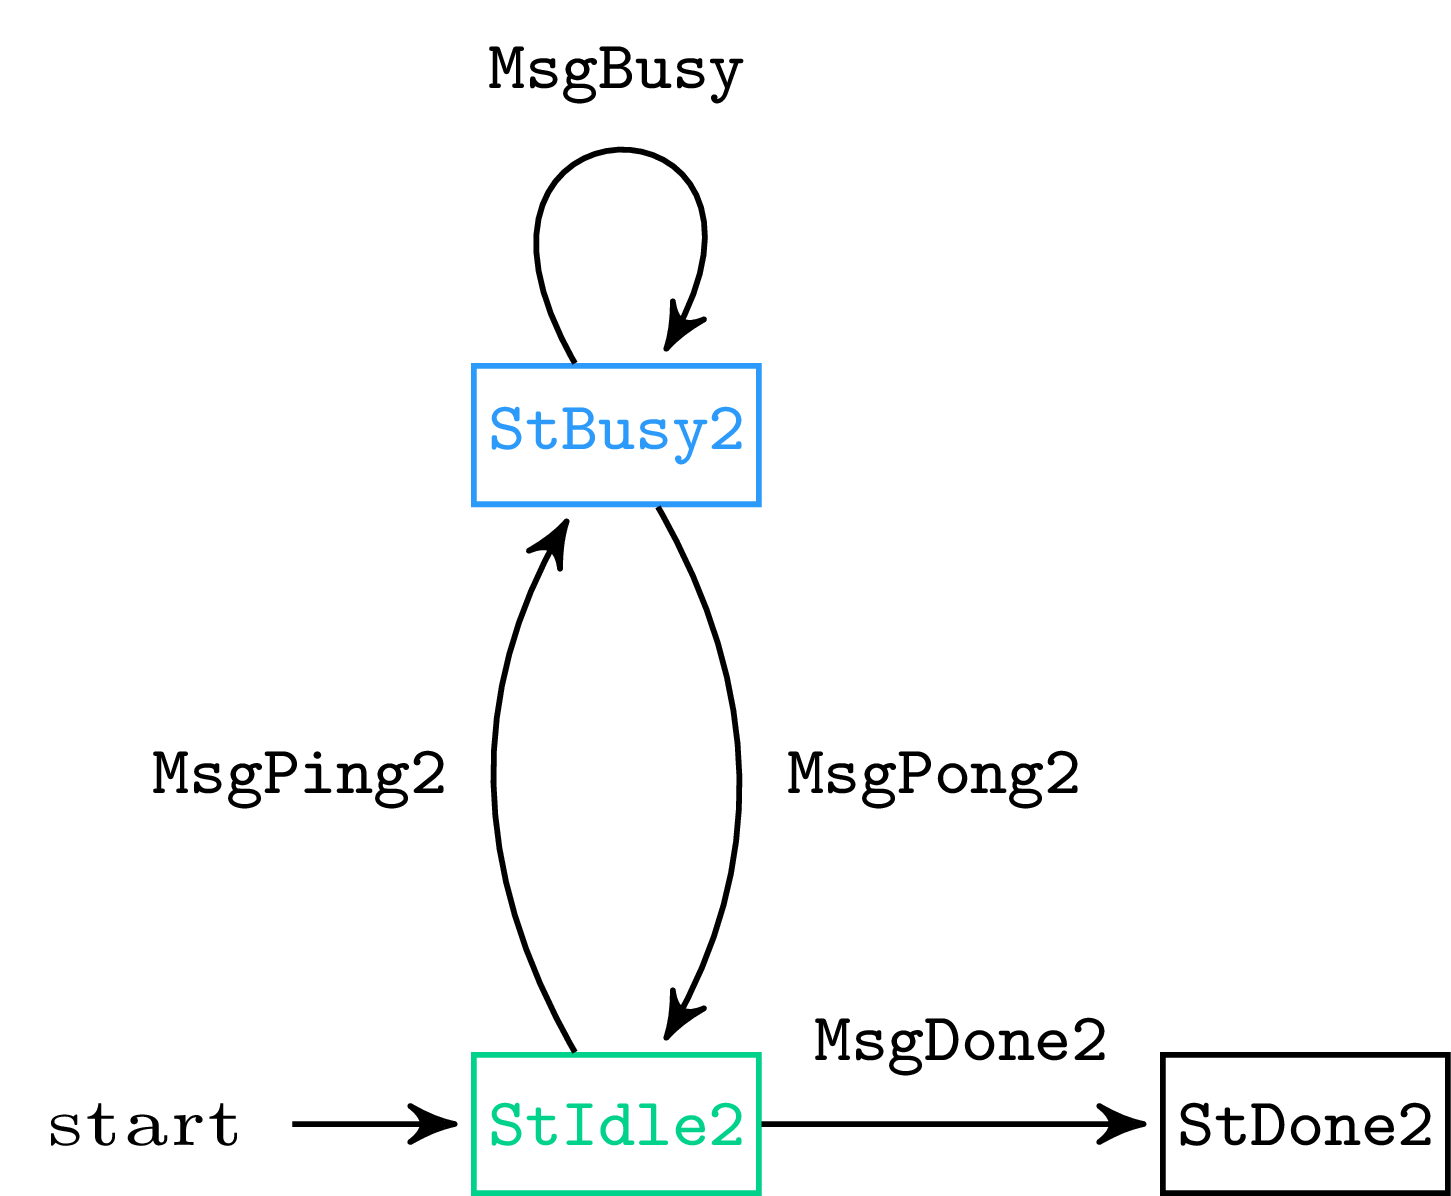
\includegraphics{../images/ping-pong-3.png}
  \end{figure}
  \begin{minted}[stripall,bgcolor=NavyBlue!5!white,fontsize=\footnotesize]{haskell}
newtype PingPong2 = Wrap PingPong
type StIdle2 = Wrap StIdle
type StBusy2 = Wrap StBusy
type StDone2 = Wrap StDone
  \end{minted}
\end{frame}

\begin{frame}[fragile]
  \frametitle{Ping Pong v2}
  \begin{minted}[stripall,bgcolor=NavyBlue!5!white,fontsize=\footnotesize]{haskell}
instance Protocol PingPong2 where
  data Message PingPong2 from to where
    MsgPingPong
      :: Message PingPong        st            st'
      -> Message PingPong2 (Wrap st)     (Wrap st')
    MsgBusy
      :: Message PingPong2 (Wrap StBusy) (Wrap StBusy)
  data ClientHasAgency st where
    WrapClient :: ClientHasAgency       st
               -> ClientHasAgency (Wrap st)
  data ServerHasAgency st where
    WrapServer :: ServerHasAgency       st
               -> ServerHasAgency (Wrap st)
  data NobodyHasAgency st where
    WrapDone   :: NobodyHasAgency       st
               -> NobodyHasAgency (Wrap st)
  exclusionLemma_ClientAndServerHaveAgency
    (WrapClient tok) (WrapServer tok') =
    exclusionLemma_ClientAndServerHaveAgency tok tok'
  ...
  \end{minted}
\end{frame}

\begin{frame}[fragile]
  \frametitle{Pipelined Ping Pong v2 Client}
  \begin{minted}[stripall,bgcolor=NavyBlue!5!white,fontsize=\tiny]{haskell}
pingPongClientPipeliend2
  :: Peer PingPong2 AsClient 'Pipelined Empty StIdle2 m Int
pingPongClientPipeliend2 =
    YieldPipelined (ClientAgency (WrapClient TokIdle))
                   (MsgPingPong MsgPing)
  $ YieldPipelined (ClientAgency (WrapClient TokIdle))
                   (MsgPingPong MsgPing)
  $ YieldPipelined (ClientAgency (WrapClient TokIdle))
                   (MsgPingPong MsgPing)
  $        collect 0
  $ \n1 -> collect n1
  $ \n2 -> collect n2
  $ \n3 -> Yield (ClientAgency (WrapClient TokIdle))
                 (MsgPingPong MsgDone)
  $        Done (WrapDone TokDone) n3
 where
  collect :: Int
          -> (Int -> Peer PingPong2 AsClient 'Pipelined q  StIdle2 m Int)
          -> Peer PingPong2 AsClient 'Pipelined
                             (Tr StBusy2 StIdle2 <| q) StIdle2 m Int
  collect !n k =
      Collect Nothing (ServerAgency (WrapServer TokBusy))
    $ \msg -> case msg of
        MsgBusy               -> collect     (n+1) k
        (MsgPingPong MsgPong) -> CollectDone      (k n)
  \end{minted}
\end{frame}

\begin{frame}[fragile]
  \begin{minted}[stripall,bgcolor=NavyBlue!5!white,fontsize=\footnotesize]{haskell}
data TerminalStates ps where
  TerminalStates :: forall ps (st :: ps) (st' :: ps).
                    NobodyHasAgency st
                 -> NobodyHasAgency st'
                 -> TerminalStates ps

theorem_nonpipelined_duality
   :: forall ps (pr :: PeerRole) (initSt :: ps) m a b.
      ( Monad m, Protocol ps)
   => Peer ps             pr  NonPipelined Empty initSt m a
   -> Peer ps (FlipAgency pr) NonPipelined Empty initSt m b
   -> m (a, b, TerminalStates ps)
  \end{minted}
  Link to the \href{https://coot.me/posts/typed-protocol-pipelining.html\#duality-for-non-pipelined-protocols}{proof}.
\end{frame}

\begin{frame}[fragile]
  \frametitle{Removing pipelining}
  \begin{minted}[stripall,bgcolor=NavyBlue!5!white,fontsize=\footnotesize]{haskell}
theorem_unpipeline
    :: forall ps (pr :: PeerRole)
                 (pl :: Pipelined)
                 (initSt :: ps) m a.
       Functor m
    => [Bool]
    -- ^ interleaving choices for pipelining allowed by
    -- `Collect` primitive. False values or `[]` give no
    -- pipelining.
    -> Peer ps pr pl           Empty initSt m a
    -> Peer ps pr NonPipelined Empty initSt m a
  \end{minted}

  Link to the \href{https://coot.me/posts/typed-protocol-pipelining.html\#removing-pipelining}{proof}.
\end{frame}

\begin{frame}[fragile]
  \frametitle{Pipelined duality}
  \begin{minted}[stripall,bgcolor=NavyBlue!5!white,fontsize=\footnotesize]{haskell}
theorem_duality
    :: forall ps (pr :: PeerRole)
                 (pl :: Pipelined)
                 (st :: ps) m a b.
       ( Monad m, Protocol ps )
    => [Bool]
    -> [Bool]
    -> Peer ps             pr  pl Empty st m a
    -> Peer ps (FlipAgency pr) pl Empty st m b
    -> m (a, b, TerminalStates ps)
theorem_duality csA csB a b =
    theorem_nonpipelined_duality (theorem_unpipeline csA a)
                                 (theorem_unpipeline csB b)
  \end{minted}
\end{frame}

\begin{frame}[fragile]
  \frametitle{Remarks}
  \begin{itemize}
    \item The duality theorem relies on 1-1 encoding of protocol messages; Non injective encodings can lead to deadlocks, or premature termination.
    \item Non injective encodings are useful!  Simultaneous TCP open.
    \item alternative agda implementation suggests that we could improve the
      \texttt{Protocol} class API.  By parametrizing it with a type family from
      protocol states to objective agency we could provide exclusion lemmas for
      all protocols rather than require it for every instance.
      \begin{minted}[stripall,bgcolor=NavyBlue!5!white,fontsize=\footnotesize]{haskell}

data ObjectiveAgency = ClientAgency
                     | ServerAgency
                     | NobodyAgency

class Protocol ps where
  data Message ps (st :: ps) (st' :: ps)
  type Agency :: ps -> ObjectiveAgency
      \end{minted}

      Open question: will this work in Haskell type system?
  \end{itemize}
\end{frame}

\end{document}
